\chapter{Konzeption und Implementierung}

Das neue Konzept, das im diesen Kapitel erklärt wird, geht es um die Migration von Datenbanken von alte webbasierte Software zur neuen Software, die auf Umbraco CMS basiert ist. Die Funktionalitäten müssen gleich bleiben.  
Das Projekt unterteilt sich auf zwei großen Paketen – Paket A und Paket B. 
Im ersten Paket wird dem Auftraggeber User Interface (UI) aufgebaut. Das Ziel ist maximale Flexibilität des Website-Besitzers zu haben und durch einfache Tätigkeiten, bestimmten Zweck zu erreichen. Man soll in diesem Bereich die Inhalt der Webseite editieren, ändern und stilisieren. Umbraco verfügt mit sogenannte „Grids“. Es dient dafür, dass man das Design der Seite manipulieren und auch die schon besprochenen Möglichkeiten ausnutzen kann. 
Es werden auch eigene Macros benutzt, in den ein Quellcode der SHOP – Komponenten hingeschrieben wird. Somit kann der Auftraggeber Macros in beliebigen Teilen der Seiten hinstellen. Umbraco – Forms werden benutzt als Formulare, damit man selber die Felder einordnen kann.
Beide Paketen werden als Startknoten aus einer Umbraco-Instanz heraus verwaltet. 
Paket B ist als Kern der Seite dargestellt. Das ist eigentlich das Online-Bestellsystem. Hier ist es wichtig, dass eine unkomplizierte, bedienbare, reibungslose und flexibel Umgebung aufgebaut wird. Das System besteht aus drei Hauptkerne:
 
\begin{itemize}	
	\item Bestellsystem
	\subitem Kundenverwaltung (Anmeldung, Kundenbereich, Kommunikation)
	\subitem Artikelverwaltung
	\subitem Auftragsverwaltung
	\item E-Mail-Verwaltung
	\subitem E-Mail-Vorlagen anlegen, editieren, löschen
	\item Umsatzerfassung
	\subitem Umsatzübersicht nach Monat und Jahr
\end{itemize}

\section{Aufbau vom Umbraco}

Wie oben schon erklärt wurde, ist Umbraco \cite{Wahlberg2011} ein Content Management System, das flexibel und Benutzerfreundlich ist. Damit man bessere Verständnis hat, worum es geht, wird es in diesem Unterkapitel erläutern. 

User Interface von Umbraco ist auf drei Teilen verteilt. Erste Teil ist Hauptfunktion bzw. Setcion. Dort befinden sich die Hauptoptionen: Content, Media. Settings, Developer, Users, Members, Forms.
Damit einen klaren Unterschied zwischen „Member“ und „User“ gemacht wird, werden die beiden Begriffe erklärt. „User“ ist jemand, der Zugriff zu „Umbraco-Backoffice“ hat und dort hat bestimmte Rechte. 

Ein Member wird von Umbraco für die Registrierung und Authentifizierung eines externen Besuchers benutzt. Das sind Leute, die nur Front-End benutzen dürfen. 
Man kann auch „Custom Setcion“ erstellen, womit wir uns im weiteren Kapitel beschäftigen. 

Nächste Teil ist Unternavigation oder auch Tree genannt. Alle Unteroptionen stehen dort. Jede Hauptfunktion hat ihre eigenen Unteroptionen.
Zugehörige Funktionalitäten der Unteroptionen (Trees) werden betrachtet.

\begin{itemize}	
	\item\textbf{Trees vom Content-Section:} In diesem Tree befinden sich alle Seiten, die im Website Front-End erschienen werden können. Dort steht auch Recycle Bin, oder auch Papierkorb genannt. So kann man die gelöschte Seite zurücksetzen. 
	\item\textbf{Trees von der Media-Section:} Hier stehen alle Videos und Bilder zur Verfügung.
	\item\textbf{Trees vom Settings-Section:} In diesem Tree befindet sich Moglichkeiten CSS, JavaStript, Document Types und zugehörige Templates. PatialView ist auch dort. Es hat eine Übertragungsfunktion von Backend zum Frontend.
	\item\textbf{Trees vom Developer-Section:} Hier stehen zur Verfügung Trees, die den Entwickler ermöglichen, bereits erstellte Seiten weiter zu entwickeln. Das wird durch Data Typ, Macros, Packages, Relation Types, XSLT Files und Partial View Macro Files ermöglicht.
	\item\textbf{Trees vom User:}In diesem Bereich stehen die Benutzer, die mit bestimmtem Rechten Umbraco-Backend benutzen dürfen. Zu einem bestimmten User können verschiedene Rechte abgegeben werden. 
	\item\textbf{Trees vom Member-Section:} Hier sind Benutzer, die Frontend benutzen dürfen.
	\item\textbf{Trees vom Forms-Section: } Hier kann man leicht verschiedene Arten von Formularen erstellen.		
\end{itemize}

Der dritte Teil vom Umbraco-Backoffice ist der Editierbereich. Dort werden alle Eigenschaften von jeweiligen Tree-Optionen dargestellt.

Im Abbildung \ref{fig:Umbraco Backoffice} kann man sehen, wie Umbraco-Backoffice aussieht.
\begin{figure}[h]
	\centering
	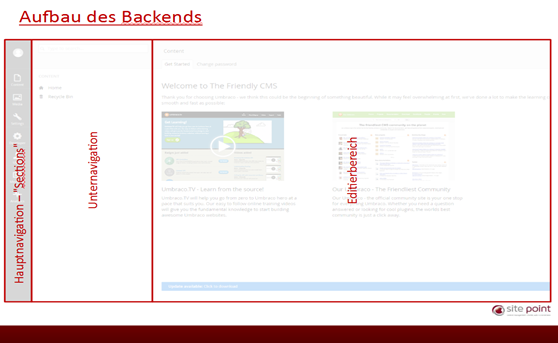
\includegraphics[width=1\linewidth]{Graphics/UmbracoBackend.png}
	\caption[Umbraco Backoffice]{Übersicht vom Umbraco-Backoffice}
	\label{fig:Umbraco Backoffice}
\end{figure}

\pagebreak
\section{Paket A}
Um der Auftraggeber mehr Flexibilität zu haben, die Frontend-Seite zu editieren, werden "Grids" - Rahmen verwendet. Grid enthält zwölf Spalten. Man kann diese Spalten zusammen binden. So ist Möglich, die Seite auf beliebige Teilen verteilt zu werden, wie im Abbildung \ref{fig:GridsLayout} gezeigt wird.

\begin{figure}[h]
	\centering
	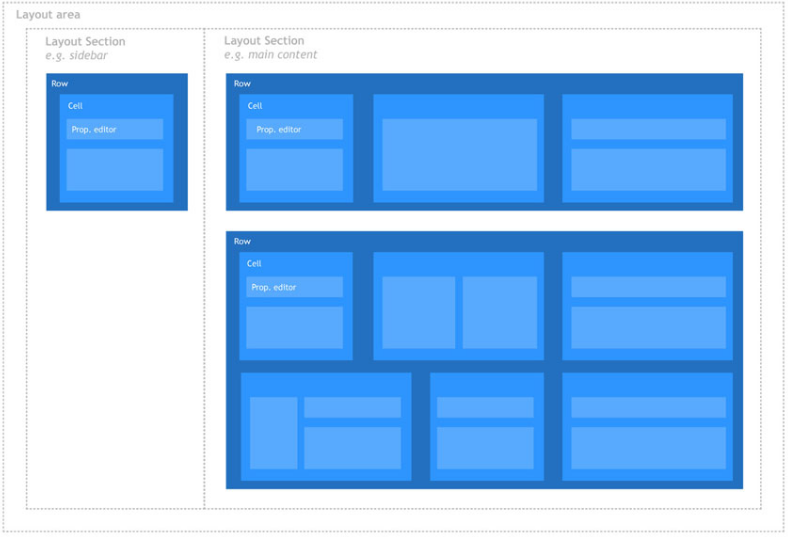
\includegraphics[width=1\linewidth]{Graphics/GridsLayout.png}
	\caption[GridsLayout]{Übersicht vom Umbraco-Grids}
	\label{fig:GridsLayout}
\end{figure}

 Im Grid kann man eigene Einstellungen machen. In dieser Arbeit werden nur zwei Beispielen gezeigt, wie Grids verwendet könnten: Die Farbe und die Größe vom Schrift ändern. "Controls" wie "Rich text editor", "Image", "Quote", "Macro"... Für angefordertes Ziel werden Rich text editor und Macros verwendet. Man kann Macros auch im Rich text editor benutzen. Das wird im späteren Kapitel gemacht. Jetzt erden nur die schon besprochene Beispiele. Sie werden im Stylesheets unter "rte" eingegeben. Im Abbildung \ref{fig:StylingGrind} kann man sehen wie CSS-Befehle im Umbraco geschrieben werden können.
     
     \begin{figure}[h]
     	\centering
     	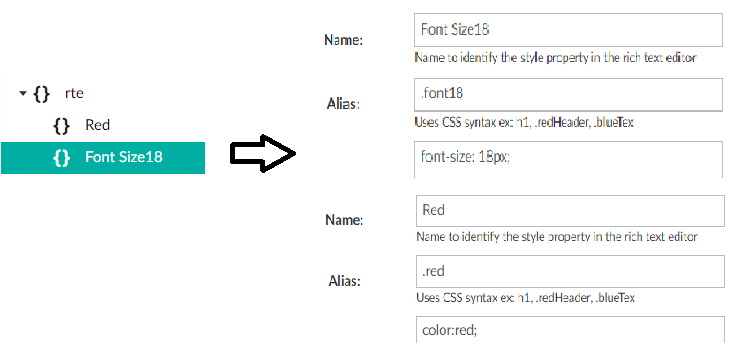
\includegraphics[width=0.6\linewidth]{Graphics/StylingGrind.png}
     	\caption[StylingGrind]{Styling vom Umbraco-Grids}
     	\label{fig:StylingGrind}
     \end{figure}
     
Über Rich text editor kann man den Text auch editieren, aber nur mit festen Optionen. 
Diese Stylesheet sind im Richtext edior integrierbar, somit kann Auftraggeber die Schriftart und Farbe ändern. 

\section{Kundenverwaltung}
Die Kundenverwaltung fasst den ganzen Bereich um, der sich um die Kunden bezieht. Mehr wird es in nächster Unterkapitel erfahren.

\subsection{Kundenerfassung}
1. Das angestrebte Ziel ist, dass der Kunde sich registrieren kann. Die Registrierung muss gesichert und individuell sein. Damit die Registrierung zuverlässig ist, muss nach den folgenden Regeln gehalten werden: Vertraulichkeit, Integrität, Verfügbarkeit und Authentizität.
Ein \ac{PIN} lässt sich in E-Mail des Kunde zusenden. So wird sichergestellt, dass die Kunde eine gültige E-Mail hat. Nach der Registrierung wird überprüft, ob die E-Mail schon existiert. Wenn ja, das Prozess wird storniert und eine Nachricht erscheint, in der geschrieben ist, dass der Kunde diese E-Mail schon verwendet. 
Der Auftraggeber entscheidet, ob der sich registrierten Kunde bestellen darf oder nicht. Danach kann der Benutzer sich mit dem PIN und die E-Mail anmelden. 
Die Kundenverfassung wird durch Member \ac{API} von Umbraco realisiert. 
Wie schon erläutert wurde, ist Umbraco auf ASP.NET basiert. Damit kann man vom CMS unterschiedliche „Services“ benutzen. Ein davon ist „MemberService“. Das ist direkte Kanal zu dem MemberAPI. Es ist in den „Services property“ von dem „SurfaceController“ zu Verfügung gestellt. 
Die Registrierung wird via ASP.Net Code und Media API programmatisch erstellt. Das ist eine komplexe Methode, in der vielfältige Dateien benötigt werden: (SurfaceController, Model, PartialView und Source Datei, in der View-Methoden über eine Aufruf-Funktion aufgerufen wird). Die benötige Information, die wir zu der Registrierung brauchen, wird im „Model“- Datei geschrieben. 
In der Datei „Model“ stehen „Model Properties“. Das sind Parametern, mit denen man arbeitet. Einfach erklärt, über das Model werden die Properties von „Partial-View“ zu dem „SurfaceController“ oder umgekehrt übertragen.
„SurfaceController“ ist der „Autobahn“ zu der Umbraco-Datei. Das ist ein \ac{MVC}, das mit dem Umbraco interagiert wird. Es wird von der Bibliothek Umbraco.Web.Mvc.SurfaceController geerbt. 
Über „PartialView“ werden die Verbindungen zwischen Kontakt Formular und „Model Properties“ geschehen. Das ist eigentlich eine Teilansicht, die von Umbraco Frontend benutzt wird. Dort ist Umbraco \ac{UI}. 
Folgende Abbildung \ref{fig:Registrierung} ergibt bessere Verständnis wie die obengenannten Begriffe zu einander stehen.

\begin{figure}[h]
	\centering
	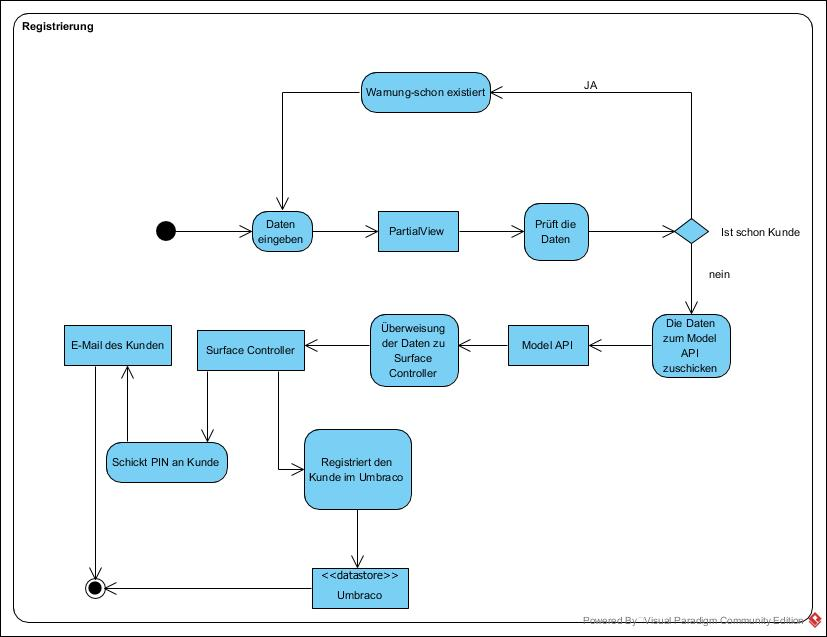
\includegraphics[width=1\linewidth]{Graphics/Registrierung.JPG}
	\caption[neues Konzept: Registrierung]{Neues Konzept zum Registrieren}
	\label{fig:Registrierung}
\end{figure}

Diese Möglichkeit vom Umbraco erlaubt den Benutzer sehr leicht und bequem in dem Server anzumelden oder sich zu registrieren.
In Anhang - Kundenerfassung kann man sich übersichtlicher genau anschauen, was es genau gemacht wird, damit diese Anforderung erfüllt wird.

\pagebreak

\subsection{Kundeansicht}
Für Erleichterung des Kunde stehen auf einer Seite alle Möglichkeiten, die der Kunde hat: 

\begin{itemize}	
	\item Neue Bestellungen abgeben, aktuelle und vorherige Bestellungen ansehen
	\item Neue Nachricht schreiben und alte Nachrichten ansehen.
	\item Wichtige Information zu beachten
	\item Individuelle Information vom Auftraggeber.
\end{itemize}
1. Der Kunde bekommt einen PIN an seinem E-Mail. Die Listings \ref{lst:PINgenerator} und \ref{lst:EmailSchicken} ermöglichen den PIN, obwohl er vom Kunde nicht eingegeben wurde, direkt zur Kundes E-Mail zugechiskt zu werden.

\begin{lstlisting}[caption={JavaScript PIN Generator}, label=lst:PINgenerator]
function myFunction() {
document.getElementById('newInput').setAttribute('Value', Math.floor((Math.random() * 9000) + 1000));
}window.onload = myFunction;
\end{lstlisting}


2. Nach der Registrierung sieht der Kunde eine neue Seite. Dort kann er die obengenannten Optionen verwenden. 
Wenn der Kunde neue Bestellung tätigen will, wird ein neues Fenster geöffnet, in dem er erwünschten Artikeln wählen und bestellen kann. Die gewählten Produkte werden in den Datenbanken gespeichert. Von dort werden sie als vergangene Bestellungen verwendet. Das selben Prinzip steht auch für die Kommunikation zwischen den Auftraggeber und den Kunden. Wenn eine Nachricht geschrieben wird, wird sie in den anderen Datenbanken gespeichert. 
Vom Umbraco wird die Information direkt zu den Kunden gesendet. 
Der Auftraggeber, so wie der Kunde, können von der Datenbank die Bestellungen und die Nachfragen ansehen. In den weiteren Kapitel wird detailliert erklärt wie die Kommunikation und die Aufträge funktioniert.
3. Nach angefordertes Ziel wird den Kunde Profile-Seite über Member abgebildet. Das Bedeutet, dass diese Seite ist nur zum jeweiligen Kunde personalisiert. Die Abbildung wird über memberId geschehen. Es wird ein Filter erstellt, durch das diese Personalisierung erreichen wird. memberId befindet sich im umbraco-Member Datenbank.
Das, was im Kundenansicht gemacht wurde, ist Verwendung von Macros und Grids. 
Damit man besser versteht, worum es geht, wird folgenden Abbildung \ref{fig:kundenansichtNew} erstellt. 

\begin{figure}[h]
	\centering
	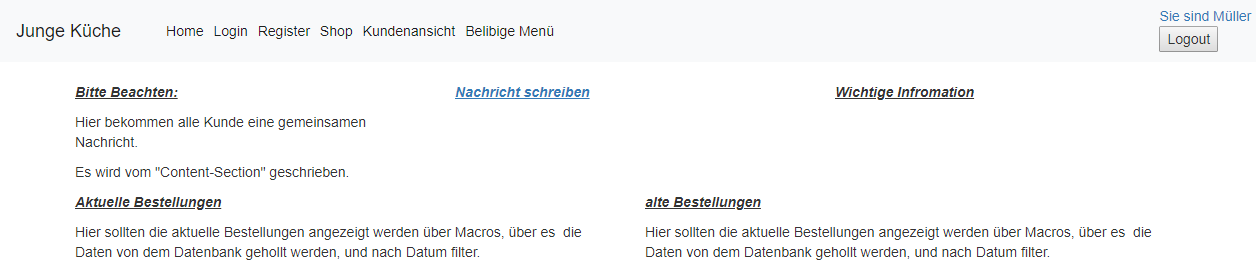
\includegraphics[width=1\linewidth]{Graphics/kundenansichtNew.png}
	\caption[Kundeansicht]{Kundeansicht}
	\label{fig:kundenansichtNew}
\end{figure}
Über ein Macros, das man im Listing \ref{lst:macroKundenansicht} anschauen kann, ist es Möglich die Meldungen vom Auftraggeber unter "Wichtige Information"  zu sehen. Im Macro ist eine Methode schrieben, über sie wird die Übertagung vom Member-Section zum Content-Section ermöglicht wird. Abbildung \ref{fig:kundenansichtNew} zeigt, wie der Auftraggeber zu dem Kunde eine Informationsmeldung von Member-Bereich schickt.
\begin{figure}[h]
	\centering
	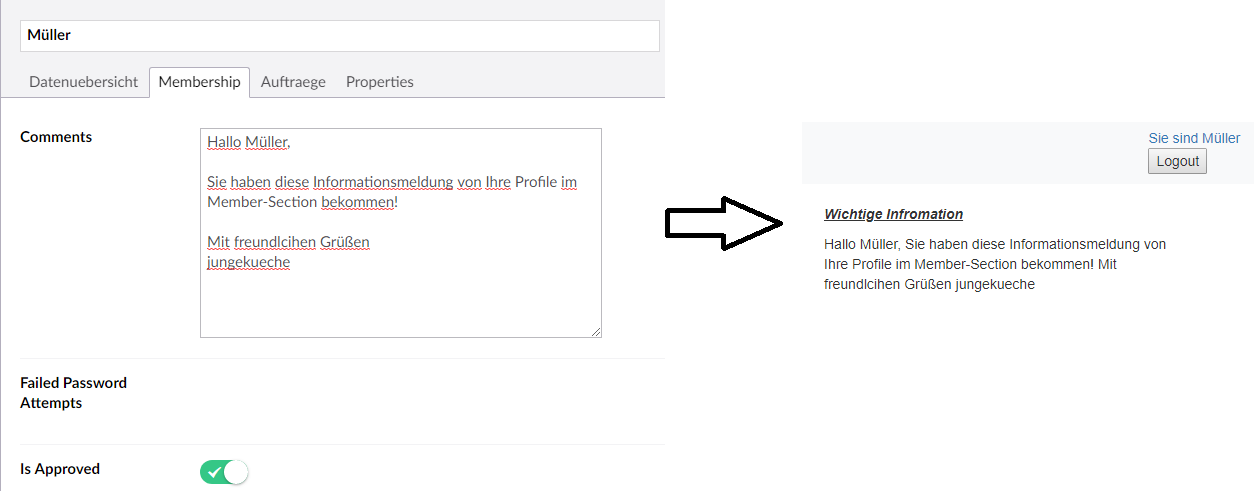
\includegraphics[width=1\linewidth]{Graphics/kundenAnsichtWichtInf.png}
	\caption[Kundeansicht]{Übertragung der Informationsmeldung von Member-Section zu Kundenansicht}
	\label{fig:kundenAnsichtWichtInf}
\end{figure}
\pagebreak
\begin{lstlisting}[caption={Macro zum Kundenansicht}, label=lst:macroKundenansicht]

@inherits Umbraco.Web.Macros.PartialViewMacroPage


@{
	var memberID = ApplicationContext.Current.Services.MemberService.GetByUsername(Membership.GetUser().UserName);
	var info = memberID.Comments;
}
@info
\end{lstlisting}

Das Kontaktfenster und allgemein die Bestellungen werden im weiteren Unterkapitel erläutert. Das gesamte Bild wird im Abbildung \ref{fig:KundenansichtNeu} dargestellt.

\begin{figure}[h]
	\centering
	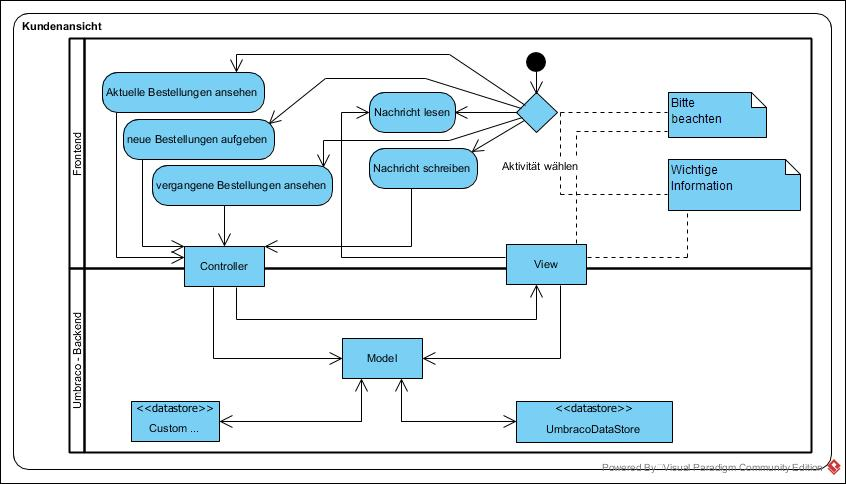
\includegraphics[width=1\linewidth]{Graphics/KundenansichtNeu.jpg}
	\caption[Funktionalität von Kundenansicht]{Funktionalität von Kundenansicht}
	\label{fig:KundenansichtNeu}
\end{figure}

\subsection{Auftraggeber-Ansicht}
  
1. Mithilfe vom Umbraco-Member-Section kann der Auftraggeber seine Kunde filtern. Es gibt eingebaute Einstellungen, wie ListView. Durch diese Möglichkeit ist man kann die Kunden im Member-Bereich filtern, nach dem Name suchen oder löschen. Es kann auch zusätzliche Properties erstellt werden. Diese Properties können über extra Attribut im Model-Datei mit dem Frontend verbunden werden.
Hier wurden neuen Tabs und Properties srtellt. Als Beispiele wird Tab-"Datenuebersicht" gegeben. Dort befindet sich nur ein Property "Ort". Im Tab-Membership ist "Password" auch ein Beispiel, aber man kann mehrere einbauen. Abbildung \ref{fig:auftraggeberAnsichtDaten} stellt dieses Tab und zugehöriges Property dar.

\begin{figure}[h]
	\centering
	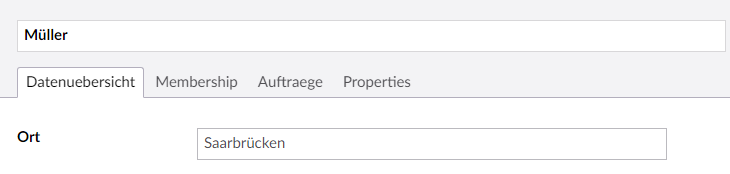
\includegraphics[width=1\linewidth]{Graphics/auftraggeberAnsichtDaten.png}
	\caption[Kundeansicht]{Beispiel zur Erstellung eines extra Tab und Property}
	\label{fig:auftraggeberAnsichtDaten}
\end{figure}
 Wie schon erläutert wurde, ist ein Macro erstellt, durch das die Information zum jeweiligen Kunde Zugeordnet ist. 

Um die Migration problemlos durchgeführt zu werden, muss man eine neue Zuordnung im Member-Bereich realisieren. Die neue Properties müssen zu den alte übertragene Attributen von der Member-Datenbank zustimmen. Mehr dafür wird im Unterkapitel "Übersicht" erläutert.  
\subsection{Kommunikation}

In diesem Kapitel wird beschrieben, die Kommunikation zwischen dem Auftraggeber und dem Kunde. Als Anforderung wird eine Übersichtliche Kommunikationsmethode mit Filtern (gelesen, nach Kunden suche...) festgestellt.



\section{Artikelverwaltung}
\subsection{Erfassen, editieren und löschen}

In der vorgegebenen Aufgabe muss den Online-Editor mit zwei Kategorien sein - Arrangements und Artikel-Standard. Diese müssen zu den zugehörigen Webseiten gekoppelt werden. Als Anforderung steht, dass Artikel-Verwaltung einfacher verwaltet werden kann und die Artikelseite der Webseite soll direkt mit dem Artikel gekoppelt sein. In der alten Seite ist die Artikel-Verwaltung nicht mit den zugehörigen Seite gekoppelt. Migration ist nicht angefordert.

Das betrachtete Ziel wird über Macros, PetaPoco-Datenbank und Umbraco vorgegebene Funktionen. Zuerst wird Umraco ListView verwendet, damit die erstellte Artikel sich im Umbraco-Content-Section unter einer gemeinsamen Unteroption befinden. Dazu ist auch vorgegeben, dass den neuen erstellten Artikel direkt editiert werden kann. Abbildung \ref{fig:ArtikelVerwaltung} zeigt übersichtlicher wie die Artikel-Verwaltung aussieht.

\begin{figure}[h]
	\centering
	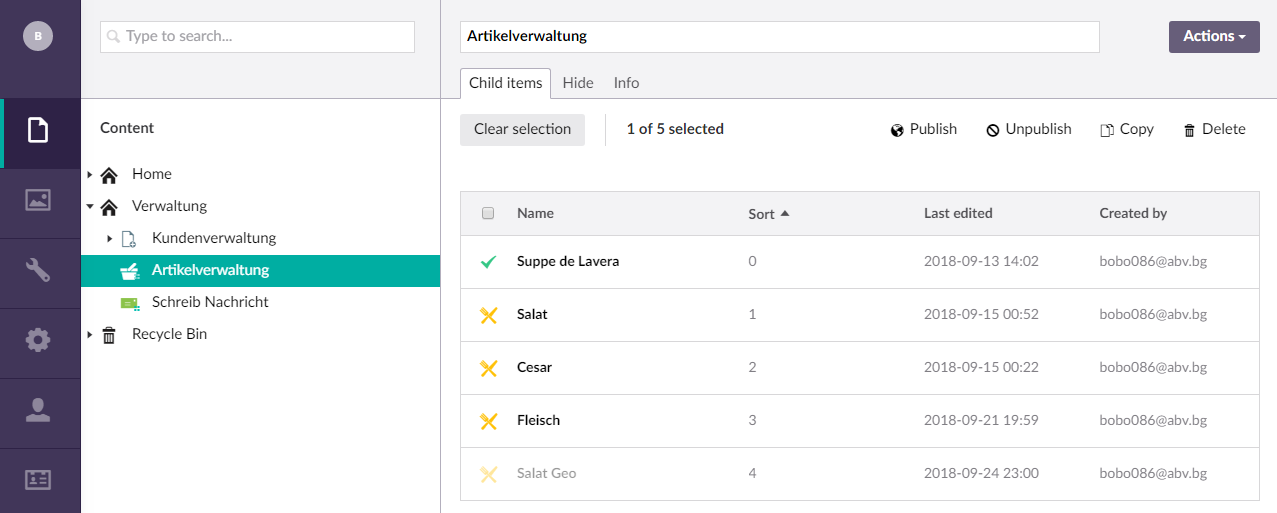
\includegraphics[width=1\linewidth]{Graphics/ArtikelVerwaltung.png}
	\caption[ArtikelVerwaltung]{Übersicht der Artikel-Verwaltung}
	\label{fig:ArtikelVerwaltung}
\end{figure}

Wenn der Artikel "unpublish" ist, kann er nicht im Frontend verwendet wird. Wenn die Artikel schon erstellt sind, wird ein Quellcode im Macros programmiert. Diese Macros werden im schon besprochenen Grids integriert, über die die Inhalt der Artikel zum Frontend übertragen wird. 
Die Inhalt wird nicht nur mit den Webseiten, sonder auch mit dem Shop-Menü gekoppelt. So wird Selbständigkeit des Auftraggeber verbessert. In der nächsten Abbildung wird gezeigt, wie mit der Erstellung von einem Artikel, werden seinen Daten sowohl im zugehörige Seite, als auch in der Shop-Menü gekoppelt.
 
 hier Abbildung
Wenn der Kunde registriert ist, kann er die von dem Auftraggeber eingegebene Artikel aus dem Shop wählen. Nach der Bestellung werden die Daten in der Datenbank "Artikel" gespeichert. Gleichzeitig werden diese Daten zusammen mit dem Kunden Daten auch im Datenbank "Auftraege" gespeichert. 




\section{Auftragsverwaltung}
\subsection{Übersicht}

Das vorgegebene Ziel ist eine Übersicht über die Aufträge und Nachrichten. Diese Ansicht soll in einer eigenen Umbraco-Section umgesetzt werden. Die Artikeldatenbank soll von Access nach SQL transportiert werden. Es muss eine neue Zuordnung zu Umbraco-Member geben.

Das vorgeschlagene Konzept umfasst die Migration von Access Datenbankdatei, Erstellung von neue Custom-Section. 

1. Um ein neues Section aufgebaut zu werden, braucht man zuerst in einer Klasse-Datei, Methoden von den Bibliotheken "umbraco.buisnesslogic" und "umbraco.interfaces" aufzurufen. Über "Application"-Methode und "IApplication"-Interface. Somit wird die Custom-Section erstellt. Wenn das fertig ist, wird die Übersicht über AngularJS-Controller und HTML erstellt. Diese Dateien werden zu dem API-Controller referenziert. In diesem Controller werden die eigentliche Funktionalitäten von Custom-Section realisiert. Mithilfe dem API-Controller werden die Daten über Model-Attributen von schon erstellter Datenbank "Auftrage" zur Verfügung gestanden, die schon im vorherigen Unterkapitel erwähnt wurde. Die Datenbanken werden über PetaPoco erstellt. Allgemein wird die Erstellung vom Custom-Section in folgender Abbildung dargestellt.

Abbildung
 
2. Wie es angefordert wurde, soll eine Migration von Access-Datenbank zu Umbraco. Das angestrebte Ziel ist, dass die alten Daten in der neuen zugehörigen Datenbank gespeichert werden. Die neue betrachtete Datenbanken sind Custom-"Artikel" und "Umbraco-Member". 
Nach tiefer Recherche wird ein Konzept erstellt. 
Grundsätzlich stehen im Umbraco Member-Section \cite{OurUmbraco2018} drei Unteroptionen - Members, Member Types und Member Groups.
Im Member Type wird die Einstellungen (Properties) des Members aufgebaut. Dort wird eine neue Member Type mit extra Properties erstellt. 
Folgendes Konzept ist basiert auf der Erwartung, dass die Datenbanken von Access auf CSV-Format konvertiert sind. Das Bedeutet, dass die Accsess-Datenbankformat Datei auf einer Text-Datei umgewandelt wird. Somit kann man die Methode "StreamReader" nutzen.
Um das vorgegebene Ziel realisiert zu werden, braucht man ein SurficeController erstellen, das die Übertragung leitet. 
Umbraco verfügt mit spezielle "Autobannen", durch die möglich ist die Manipulation von festgelegte Sections im Umbraco. Man nennt diese "Autobannen" - "Services". Sie werden über "ApplicationContext" aufgerufen. In diesem Fall wird "MemberService" genutzt.
Damit die Datei gelesen wird, wird die Funktion "StreamReader" verwendet. Somit wird die gelesene Datei in einer Variablen gespeichert. Von dieser Variablen wird mithilfe von dem Befehl "split" in einem Array gespeichert. Jeder Teil von dem Array wird über MemberService Befehle und Methoden im Umbraco Members gespeichert. Im Anhang \ref{lst:migrationsController} steht das Quellcode, um man besseres Vorbild zu haben.
Die Abbildung stellt dar, wie dies Prozess durchgeführt wird.

Abbildung 

Wenn die Kundendaten schon übertragen wurden, kann man das selben Prinzip der Migration für die Artikel benutzen. Hier wird als Ziel statt MemberServices - Datenbank "Artikel"-Datenbank  verwendet. Nach der Umwandlung von Access-Datenbankdatei auf CSV-Format, wird diese Datei über die Methode "StreamReader", danach ist die Information im ein Array gespeichert. Über API-Controller werden die Daten im "Artikel"-Datenbank übertragen. In Listing \ref{lst:DBInputArtikel}

\begin{lstlisting}[caption={Datenbank "Artikel" - Transfer}, label=lst:DBInputArtikel]

var setArtikel = new Artikel();
var db = new PetaPoco.Database("umbracoDbDSN");
setArtikel.kundeID =_split[0];
setArtikel.bezeichnung = _split[1];
setArtikel.beschreibung = _split[2];
setArtikel.preis = _split[3];
setArtikel.art = _split[4];
setArtikel.kannWaehelen = m_split[5];

db.Insert(setArtikel);
\end{lstlisting}

\subsection{Detailansicht}

Hier wird angefordert, dass der Auftraggeber die Aufträge bearbeiten kann, den Status ändern, Positionen editieren, hinzufügen oder löschen, dem Kunden Freigaben erteilen (zum Beispiel Aussuchen der Positionen) und ein Rechnungsnummer vergeben. Diese Aktivitäten müssen in eigenen Umbraco-Section umbesetzt werden. 

Es wird wie im vorherigen Unterkapitel ein Umbraco-Section aufgebaut. Die verwendeten Datenbanken sind "Auftraege"

\section{E-Mail Verwaltung}
\section{Umsatzverwaltung}


